\documentclass{wx672beamer}

\addbibresource{bib/net.bib}
\addbibresource{bib/rfc.bib}
\addbibresource{bib/wikipedia.bib}

\begin{document}
  
\begin{frame}
  \title{Iptables Quick Tutorial}
  \author{Wang Xiaolin\\\texttt{\small wx672ster@gmail.com}}
  \titlepage
\end{frame}

\begin{frame}{What's A Packet Filter?}
  \begin{description}
  \item[A packet filter] is a piece of software which looks at the
    \code{header} of packets as they pass through, and decides the
    fate of the entire packet. It might decide to
    \begin{itemize}
    \item \code{DROP} the packet (i.e., discard the packet as if it
      had never received it),
    \item \code{ACCEPT} the packet (i.e., let the packet go
      through), or
    \item something more complicated.
    \end{itemize}
  \end{description}
\end{frame}

\begin{frame}{Why Packet Filtering?}
  \begin{description}
  \item[Control] --- allow certain types of traffic, and disallow others.
  \item[Security] --- you might not want outsiders telnetting to your Linux box.
  \item[Watchfulness] --- It's nice to tell the packet filter to let you know if anything
    abnormal occurs.
  \end{description}
\end{frame}

\begin{frame}{Packet Filter Under Linux}
  \begin{description}
  \item[iptables] talks to the kernel and tells it what packets to filter.
  \end{description}
  The iptables tool inserts/deletes rules from the kernel's packet filtering table.
\end{frame}

\begin{frame}{Quick Start}
  \begin{block}{Debian/Ubuntu users can do:}
    \begin{center}
      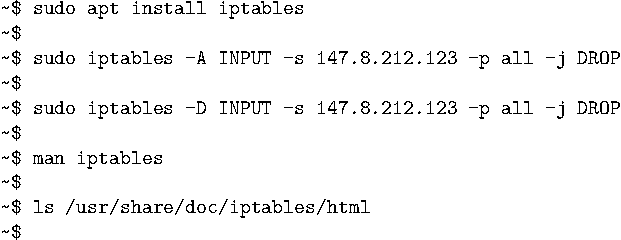
\includegraphics[width=\textwidth]{quick}
    \end{center}
  \end{block}
\end{frame}

\begin{frame}{Terminology}
  \begin{description}
  \item[Filter table] is in the kernel, contains \code{chains}.
  \item[Chains] a.k.a. firewall chains, are lists of filtering rules. The three kernel
    built-in chains are called \code{INPUT}, \code{OUTPUT}, and \code{FORWARD}.
  \item[Rules] Each rule says:
    \begin{itemize}
    \item[\code{if}] the packet header looks like this
    \item[\code{then}] here's what to do with the packet
    \end{itemize}
  \end{description}
\end{frame}

\begin{frame}{How Chains Work?}
  \begin{figure}
    \centering
    \includegraphics[width=\textwidth]{Chains}
    \caption{Chains}
    \label{fig:chains}
  \end{figure}
\end{frame}

\begin{frame}{Using iptables}
  To manage whole chains:
  \begin{enumerate}
  \item Create a \underline{n}ew chain (\code{-N}).
  \item Delete an empty chain (\code{-X}).
  \item Change the \underline{p}olicy for a built-in chain. (\code{-P}).
  \item \underline{L}ist the rules in a chain (\code{-L}).
  \item \underline{F}lush the rules out of a chain (\code{-F}).
  \item \underline{Z}ero the packet and byte counters on all rules in a chain (\code{-Z}).
  \end{enumerate}
  To manipulate rules inside a chain:
  \begin{enumerate}
  \item \underline{A}ppend a new rule to a chain (\code{-A}).
  \item \underline{I}nsert a new rule at some position in a chain (\code{-I}).
  \item \underline{R}eplace a rule at some position in a chain (\code{-R}).
  \item \underline{D}elete a rule at some position in a chain, or the first that matches
    (\code{-D}).
  \end{enumerate}
\end{frame}

\begin{frame}{Examples}
  \begin{block}{}
    \includegraphics[width=\textwidth]{exp1}
  \end{block}
\end{frame}

\begin{frame}{More Examples}
  \begin{block}{}
    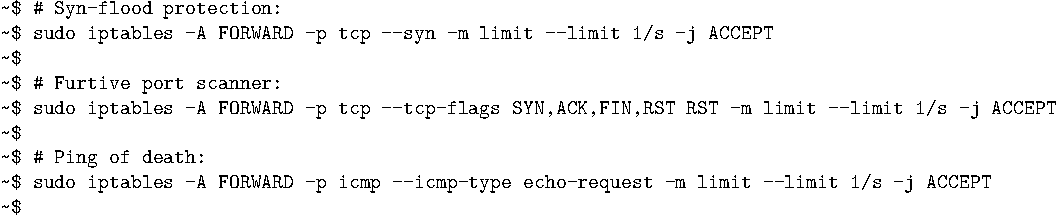
\includegraphics[width=\textwidth]{exp2}
  \end{block}
\end{frame}

\begin{frame}[allowframebreaks=.8]{References}
  \begin{refsection}
    \nocite{rfc2663, rfc3022, rfc2827, rfc1858, rfc3128, wiki:iptables, bautts2005linux,
      hunt2002tcp}%
    \printbibliography[heading=none]
  \end{refsection}
\end{frame}

\end{document}

%%% Local Variables: 
%%% mode: latex
%%% TeX-master: t
%%% End: 
